% Copyright (C) 2018 by latexstudio <http://www.latexstudio.net>
%
% This program is free software: you can redistribute it and/or modify
% it under the terms of the GNU General Public License as published by
% the Free Software Foundation, either version 3 of the License, or
% (at your option) any later version.
%
% This program is distributed in the hope that it will be useful,
% but WITHOUT ANY WARRANTY; without even the implied warranty of
% MERCHANTABILITY or FITNESS FOR A PARTICULAR PURPOSE.  See the
% GNU General Public License for more details.
%
% You should have received a copy of the GNU General Public License
% along with this program.  If not, see <http://www.gnu.org/licenses/>.
%

% !TEX root = ../latex-faq-cn.tex
% !TEX program = xelatex
% !TEX options = --shell-escape

\section{参考文献篇}


\faq{如何排版参考文献?}{}

传统的基于bibtex的参考文献生成方法:

\begin{enumerate}

\item
  准备一份 BibTeX 数据库,假设数据库文件名为 books.bib,和 LaTeX
  源代码一般位于同一个目录下。
\item
  在源代码中添加必要的命令,如 |\bliographystyle{abbrv}|,|\bibliography{books}|。假设源代码名为
   demo.tex。其中,\cs{bibliographystyle}设定参考文献的格式。
   \cs{bibliography}
  告诉系统使用哪个数据库和参考文献列在哪个位置。
\item
  写好了以上两个文件之后,我们就可以开始编译了。例如在命令行中执行以下命令
  
\begin{texinlist}
xelatex demo
bibtex demo
xelatex demo
xelatex demo
\end{texinlist}
\end{enumerate}



或者选择一个可以自动检测是否有参考文献的编辑器,如果有,它会自动执行以上四个命令,但是有时候会遇到检测不到的情况,这时你只需要清理一下辅助文件即可。

基于biblatex的参考文献生成方法,与基于bibtex的方法类似,只是文献数据处理程序需要换成biber:

\begin{enumerate}
\item 首先准备BibTeX格式文献数据库,即bib文件

\item 接着完成tex源代码,即tex文件,其中参考文献样式引入用biblatex宏包,打印文献用printbibliography命令,比如:

\begin{texinlist}
\documentclass[twoside]{article}
	\usepackage[backend=biber,style=alphabetic]{biblatex}
    \addbibresource{youbib.bib}

\begin{document}
    \section{references of alphabetic style}

	\nocite{*}

    \printbibliography
\end{document}
\end{texinlist}

\item 最后编译文档,命令如下:

\begin{texinlist}
xelatex demo
biber demo
xelatex demo
xelatex demo
\end{texinlist}

\end{enumerate}


\faq{编译参考文献后在文献引用处出现问号,或者文献的引用关键字,或者文献表不显示?}{}

这些信息都显示参文献并没有编译正确。可以从以下几个步骤进行检查和排除:
\begin{enumerate}
\item 是否正确完成了编译步骤?编译方法见上一问题

\item 检查.blg文件内容,看是否存在如下问题:

\begin{itemize}
  \item bibtex或biber是否找到样式文件?
  \item bibtex或biber是否找到文献数据库及bib文件?
  \item 数据文件是否存在问题?其中是否包含引用的文献?
  \item 引用的文献的数据是否有效?
\end{itemize}

\item 排除上述问题后,清楚辅助文件,重新进行完整编译。

\end{enumerate}



\faq{有没有关于参考文献生成的入门资料?}{}

\begin{enumerate}
\item 传统的基于bibtex的参考文献生成方法的资料包括:

\begin{itemize}
  \item lshort(从ctan下载)
  \item lshort-zh-cn(从github下载)
  \item btxdoc(从ctan的bibtex宏包下载)
  \item btxFAQ(从ctan的bibtex宏包下载)
  \item 刘海洋和胡伟的书(可购)
\end{itemize}

\item 基于biblatex的参考文献生成方法的资料包括:

\begin{itemize}
  \item biblatex(从ctan下载)
  \item biblatex-zh-cn(从github下载)
  \item biblatex-tutorial(从github下载)
  \item biblatex-solution-to-latex-bibliography-master(从github下载)
\end{itemize}

\end{enumerate}

此外 tex exchange上面有大量关于bibtex,biblatex方面的提问和回答,很多都是前辈大佬们的精心总结,很值得一看。国内latexstudio和ctex论坛上面也有很多好的资料和内容可以详细学习。


\faq{是否可以处理非英文的参考文献?}{}

传统的基于bibtex的参考文献生成方法,中文的参考文献条目,与英文条目并没有什么差别,只是注意编码。目前处理中文推荐用xelatex 编译 utf8 编码的文件。因此中文的 bib 条目也应该用 utf8 编码。bibkey也能用中文,处理好编码格式,无殊。

基于biblatex的参考文献生成方法,支持多语言参考文献。可以利用babel等宏包实现西文文献的无缝切换,可以实现多语言共存的文献表。东亚语言的参考文献,可以利用英文文献的机制生成,基于参考文献样式的设计,可以实现中英文对照的文献表。biblatex完全既支持unicode编码,也支持其他编码,因此可以处理任何语言的参考文献。


\faq{BibTeX 参考文献数据库}{}

BibTeX 的 bib 文件是一个记录已阅文献的数据库,但是通常不建议手动编译 bib
文件,建议:

\begin{enumerate}
\def\labelenumi{\arabic{enumi}.}

\item
  使用 JabRef 或 Zotero 等文献管理工具导出 bib 文件创
\item
  使用 \href{https://scholar.google.com/}{Google Scholar} 或
  \href{https://cn.bing.com/academic}{Bing 学术}导出 bib 条目建
\end{enumerate}

引文的信息还有很多国内外网站可以获取包括:
\begin{itemize}

  \item 百度学术

  \item 搜狗学术

  \item CNKI

  \item 万方

  \item 维普

  \item Citeulike

  \item amazon

  \item nelson beebe's collection

  \item bibsonomy

  \item mathscinet

  \item acm catalog

  \item ieee catalog

  \item collection of CS bibliographies

  \item DBLP

  \item SPIRES

  \item CITING Wikepedia itself

  \item texmed

\end{itemize}


\faq{BibTeX 文献手写很困难,有没有什么工具能够生成?}{}

多数时候,我们无需自己手写 BibTeX 文献条目。从
\url{https://scholar.google.com/}、\url{https://academic.microsoft.com/}、
\url{https://cn.bing.com/academic?mkt=zh-CN}
或者期刊、数据库的网站上都能够导出 BibTeX 文献条目。 

老牌的文献管理软件
EndNote 也支持生成 BibTeX 格式的数据库,详情见
官网\url{https://endnote.com/}。 

开源软件 JabRef 甚至支持 BibTeX
文献条目的导入、导出和管理,详情见 官网\url{http://www.jabref.org/}。

Zetero 使用起来也非常方便,详情见官网 \url{https://www.zotero.org/}。

谷歌学术、知网、百度学术、万方数据库等在线数据库也是可以支持导出 .bib
文件的,至于哪家的数据条目更全,就得你自己去甄别了。


\faq{bib文件的重建}{}

用文本编辑器如Notepad++, Sublime
Text或WinEdt或专门文献管理软件JabRef,BibDesk等创建文件,改名为 ref.bib
文件,往里头添加参考文献目录。参考如下:
% \includegraphics{https://images-cdn.shimo.im/VKQ8uAycksg1zPlo/image.png!thumbnail}

在.bib文件中,可以采用 TeXStudio 提供的参考文献格式,在自行修改内容
% \includegraphics{https://images-cdn.shimo.im/0OgCsRQoufMTDJ75/1.png!thumbnail}

上面的类型有两种选择 BibTeX 和 BibLaTeX ,后者的选择更为广泛。

参考文献一般不自己书写,而是有可以直接导入。 一般直接 Google 学术搜索出来的文献或者引用知网,如下:
% \includegraphics{https://images-cdn.shimo.im/L1fAEZmW9tYDVTYT/VRI1FEC62J_C6_QSK_P0_0.png!thumbnail}

点击上图红圈的引号-\textgreater{}
% \includegraphics{https://images-cdn.shimo.im/N8tFzuXsCM8rOPjF/image.png!thumbnail}

在点击最左侧的 BibTeX -\textgreater{}
% \includegraphics{https://images-cdn.shimo.im/81Z6BGei8ycQf1uK/image.png!thumbnail}

将其复制黏贴到你的 ref.bib 文件中即可。

在知网上的文献查询需要下载安装如下软件:
% \includegraphics{https://images-cdn.shimo.im/ZsikCVGdjGIKBqSN/image.png!thumbnail}

两个都装好了之后,该软件需要自行注册登陆使用。然后打开知网,会看到如下:
% \includegraphics{https://images-cdn.shimo.im/DVEoaSyHJKwmbSjH/2.png!thumbnail}

右上角红圈圈到的就是为浏览器安装的 Zotero Connector插件,在此需要打开 Zotero 软件,点击之后显示下图,选择需要的文献。
% \includegraphics{https://images-cdn.shimo.im/w4eu1WOehS05gJ0g/image.png!thumbnail}

然后 Zotero 软件如下显示
% \includegraphics{https://images-cdn.shimo.im/VFUjYs5MvKQz522e/image.png!thumbnail}

然后文件-\textgreater{}导出文献库-\textgreater{}导出格式 BibTeX 确定保存生成的bib文件,可以将这个 bib 文件中的参考文献全部复制黏贴到你的 ref.bib 文件中,也可以单独作为一个新的bib文件,在正文区则需要添加多个bib文件就可以,用命令:

\begin{texlist}
\bibliography{test,ref}
\end{texlist}

多个bib文件用逗号分隔即可。同时为引用的参考文献需要命令 \verb|\nocite{*}| 来将未引用的文件全部排版出来。

注:百度学术、万方数据库等也支持导出 .bib文件。

\faq{如何从一个大的bib数据库中导出一个小的由当前文档引用的文献构成的bib文件?}{}

传统的基于bibtex的参考文献生成方法,可以使用 \verb|bibtool| 这一命令行工具,
可以根据 \verb|.AUX| 文件中的引用信息导出一个bib文件。

基于biblatex的参考文献生成方法,直接使用biber可以导出当前文档引用文献的bib文件,命令为:

\begin{texlist}
biber jobname --output-format=bibtex
\end{texlist}


\faq{参考文献中的特殊字符或字母}{}


参考文献信息中大体可能有几类特殊的字符或字母:

一是 \%\&\#这里键盘上直接能输入的字符,那么使用tex对特殊字符的输入方法,比如\verb|\%|,\verb|\&|,\verb|\#|。类似带重音符号的字符,也可以用花括号进行保护。

二是数学类的字符,那么使用数学环境来输入,比如\verb|$\mathbf{R}$|,\verb|$\mathbb{L}$|

三是单纯的unicode字符,那么直接输入它,比如$\phi$。但要注意要显示这些unicode字符,需要能显示该字符的字体的支持,比如 CMU Serif等。


\faq{BibTeX 不理解的作者列表}{}

BibTeX 只支持三种姓名格式: * First von Last * von Last, First * von
Last, Jr, First

多个姓名之间必须使用``and''连接,如

\begin{texlist}
author = {Knuth, Donald E. and Lamport, Leslie},
\end{texlist}

当有更多作者省略时,可以加上“and others”,比如:

\begin{texlist}
author = {Knuth, Donald E. and Lamport, Leslie and others},
\end{texlist}


\faq{BibTeX 中的大写字母}{}

英文标题中常使用的大小写方式有:

\begin{enumerate}
\def\labelenumi{\arabic{enumi}.}

\item
  Title case:
  句首字母大写,并且除冠词、连词和短介词以外的词首字母大写,这里说的``短''介词一般指不超过
  4 个字母的介词。比如``The Quick Brown Fox Jumps over the Lazy Dog'';
\item
  Sentence case:
  句首字母和一些专有名词的首字母大写,同普通的英文句子大小写方式一样,如``The
  quick brown fox jumps over the lazy dog''。
\end{enumerate}

BibTeX 根据 bst 样式文件可以将题名保留原大小写,或转为 sentence
case。所以用户在 bib 数据库中著录标题的正确方式是,统一使用 title
case,并将需要专有名词用大括号括起来。

\begin{texlist}
title = {Finite Element Methods for {Maxwell's} Equations},
\end{texlist}

注意尽量避免将一个词中个别字母用大括号括起来,如``\{M\}axwell's'',这可能会导致字母的间距有问题,建议将整个词括起来,如``\{Maxwell's\}''。

基于biblatex的参考文献生成方法,同样支持这种用花括号保护字母大小写的机制。一般情况下,文献各部分内容的大小写,会由参考文献样式来决定,当有特殊要求的时候,比如使用专有名词等,才需要采用这种保护机制。



\faq{bib文件中怎么进行注释?}{}

对于条目来说,去掉条目类型前的 @ 符号就可以将整个条目注释掉。
对于域来说,将域的名称修改为bibtex不认识的域名,就可以将该域注释掉。



\faq{bibtex中的多字母缩写}{}

有时需要从多个词构成的字符串中提取各个词的首字母,以大写形式构成一个缩写信息。在目前的latex中,无论基于bibtex的方法,还是基于biblatex的方法,均没有提供这种现成工具。但是用户可以手动提供的一个缩写信息,比如;

\begin{texlist}
author ={{National Aeronautics and Space Administration}},
shortauthor={NASA},
\end{texlist}

其中shortauthor就是author的缩写信息。缩写信息的使用则由参考文献样式决定,一般情况下,标注、缩略信息表中使用shortauthor,而参考文献表中使用author,但这些并不是绝对的,因为样式都是可以定制的。


\faq{不同 journal 给出的 bibtex 文件格式不一致,如何批量快速格式化多个.bib 文件}{}

bib文件的管理可以使用工具比如jabref等进行。而且bib文件本质上一个文本文件,因此可以利用文本处理工具进行处理,比如notepad++软件,利用搜索替换,利用正则表达式,可以进行高效修改。



\faq{制作参考文献的HTML}{}

bib文件转换为HTML,可以使用如下工具:
\begin{itemize}
  \item bibutils

  \item bibteXML

  \item bib2xhtml

  \item bib2html

  \item bibtex2html

  \item bibtex-xml-html
\end{itemize}



\faq{如何选择参考文献的风格}{}

参考文献的风格一般是期刊或会议模板指定 bst 的,作者应仔细阅读投稿要求和模板使用说明,根据规定使用合适的bst。通常有以下方式:

\begin{enumerate}
\item
  在文档中声明 |\bibliographystyle{ieeetran}|
\item
  在模板的文档类选项中使用合适的参数,如 |\documentclass[authoryear]{ustcthesis}|。
\end{enumerate}

基于biblatex的参考文献生成方法,文献表的著录格式和正文中的引用标注也都是由样式文件决定的,不同于bibtex的bst文件,biblatex的样式使用bbx和cbx为后缀名。选择某种文献风格(规范/标准),就是选择符合该风格的样式,比如要采用ieee的风格,在导言区做如下声明:

\begin{texlist}
\usepackage[backend=biber,style=ieee]{biblatex}
\end{texlist}

其中,选择的 \verb|style=ieee|样式,实质上是使用了ieee.bbx和ieee.cbx两个样式文件。



\faq{创建参考文献风格}{}

BibTeX 的风格文件 bst 是使用一种后缀语言写的代码,如果对编程能力比较自信的话,可以阅读 BibTeX 的文档 btxdoc 和 btxhak,btxbst.doc 文件提供了标准 bst 风格的代码注释,另外还可以阅读 ttb 和 The LaTeX Companion 等资料。如果不习惯 bst 的编程语言,可以使用 custom-bib 工具,在命令行下运行latex makebst,回答一系列问题生成自己的bst。

另外还可以考虑使用 biblatex,它提供更方便的接口用于自定义参考文献格式。
基于 biblatex 的参考文献生成方法,文献格式由参考文献样式文件控制,即前面提到过的bbx和cbx文件。尽管biblatex 的参考文献样式定制相对简单,但作为一般用户,首先要做的是查看是否有现成的参考文献样式可以使用,因为除了biblatex自带的各种标准样式外,还有更多第三方提供的样式可用,比如 trad-usrt,ieee,apa,mla,gb7714-2015 等等。实在没法使用现成资源,再考虑创建 biblatex 的参考文献样式,具体的方法可以参考 biblatex 手册及其\href{https://github.com/hushidong/biblatex-zh-cn}{中译版}。





\faq{怎么在一个文档中生成多个参考文献表}{}

传统的基于bibtex参考文献生成方法,natbib宏包与Donald Arseneau和Niel Kempson编写的chapterbib宏包兼容,该宏包允许在一个文档内有多个独立的参考文献列表。通常用法是一本书的各章有独立的参考文献列表,尤其是在各章由不同作者独立编写时。此外还有multibib,splitbib,bibunits等宏包可以使用,各个包功能特性略有不同,适用场合也略有不同。

基于biblatex的参考文献生成方法,可以由printbibliography命令在文档任意位置生成任意数量的文献表。就分章文献表而言,biblatex提供了refsection环境来划分参考文献节,每一节都可以生成一个独立的文献表:

\begin{texlist}
\chapter{one}
\begin{refsection}
citation for chapter one\cite{bibkey1}
\printbibliography
\end{refsection}

\chapter{two}
\begin{refsection}
citation for chapter two\cite{bibkey2}
\printbibliography
\end{refsection}
\end{texlist}

其中,两章内容分别生成一个文献表,第一章的文献表打印文献bibkey1,第二章打印bibkey2。

\faq{按照章节分开参考文献条目}{}

参见上一问题。

传统的基于 bibtex 的参考文献生成方法,可以使用chapterbib,bibnunits等宏包。

基于 biblatex 的参考文献生成方法,可以使用refsection,refsegment等环境。


\faq{插入参考文献列表有几种方式?如何定义其样式?如何定义正文引用样式?}{}


传统的基于bibtex参考文献生成方法,文献表样式由bst文件决定,定义格式就是要设计bst文件,引用样式通常由使用的latex宏包决定,比如natbib等。

基于biblatex的参考文献生成方法,使用 \verb|\printbibliography| 打印参考文献的完整信息列表,利用 \verb|\printbiblist| 打印参考文献的缩略信息列表。

列表内部各条目的著录格式以及整个列表的段落格式由参考文献样式决定。其中整个列表的段落格式由 \verb|\defbibenvironment| 定义的环境控制。而正文的引用样式由cbx样式文件决定。


\faq{如何在文献表中打印未引用的文献}{}

科技论文通常要求参考文献表中的文献必须在正文中引用,但是在某些特殊情况下仅需要列出 bib 数据库中的文献,可以使用 \verb|\nocite{*}| 命令列出调用的bib中所有条目,或者使用类似 \verb|\nocite{ref1,ref2,ref3}| 命令列出需要显示的条目。

基于biblatex的参考文献生成方法同样支持这种机制,可以利用 nocite 命令将未在正文引用的文献引入到文献表中。


\faq{如何分开打印文档中引用和未引用的文献表}{}

基于biblatex的参考文献生成方法可以利用分类筛选机制来完成,比如利用category来实现。


\faq{同一位置引用多篇文献以及分组文献集合}{}

只需要将多篇文献的bibkey用英文半角逗号分隔写在一个cite指令的选项里即可。如:

\begin{texlist}
\cite{knuth84,lamport86}
\end{texlist}

基于biblatex的参考文献生成方法,同样支持这种逗号分隔列表的机制。比如:
\begin{texlist}
\cite{bibkey1,bibkey2,bibkey3,bibkey4}
\supercite{bibkey1,bibkey2,bibkey3,bibkey4}
\parencite{bibkey1,bibkey2,bibkey3,bibkey4}
\textcite{bibkey1,bibkey2,bibkey3,bibkey4}
\end{texlist}

当同一位置引用的多篇文献需要构成一个集合时,即在文献表中以分组的形式集中在一起打印,且标注标签以集合的形式仅显示一个。

传统的基于bibtex参考文献生成方法,是利用mcite宏包,使用如下命令:

\begin{texlist}
\cite{paper0,paper1,*paper2,*paper3}
\end{texlist}

其中*符号表示将paper2,paper3与paper1构成集合打印且标注只有一个标签,如果paper0标签为[1],那么paper1,paper2,paper3构成的集合的标签为[2]。

基于biblatex的参考文献生成方法,支持类似的机制,但命令略有不同,当启用mcite模块时,可以使用如下命令:

\begin{texlist}
\mcite{paper0,set1,*paper1,*paper2,*paper3}
\end{texlist}

其中:biblatex用一个set1显式的表明这是一个集合,其由后面跟着的带*号的key的文献构成。
需要注意的是,集合的著录格式由样式文件决定。



\faq{bibtex 排序和名字前缀}{}

参考文献的排序一般由参考文献样式决定。即:

对于传统的基于bibtex参考文献生成方法,排序由bst决定。

对于使用biblatex的参考文献生成方法,排序由biblatex的样式决定。

名字的前缀在排序中扮演的角色由这些参考文献样式设定。




\faq{引文的排序及压缩}{}

当在同一处引用多篇文献时,可能涉及到不同文献的排序,以及序号标签的压缩,比如[1,2,3,4]压缩成[1-4]。

传统的基于bibtex参考文献生成方法,排序和压缩取决于使用的宏包,常用的natbib宏包可以使用sort或者sort\&compress选项激活相应的排序或排序并压缩功能。

基于biblatex的参考文献生成方法,文献表的排序由sorting选项控制,而引用的标注标签中的排序则有sortcites选项控制,引用标注标签的压缩则由所采用的标注样式决定,类似numeric-comp这样带comp的biblatex 标准样式通常使用压缩方式。



\faq{引文列表(文献表)排序}{}

传统的基于bibtex参考文献生成方法,排序取决于bst,一般模板都有指定的bst,用户无需调整。但使用thebibliography环境直接写文献表的用户可能会遇到文献表排序的问题,因为bibtex只支持自己生成内容的排序,因此用户只能手动调整。

基于biblatex的参考文献生成方法,引文列表排序,由sorting选项控制,一般情况下,各个参考文献样式做了默认设置,无需调整。



\faq{在章节标题中引用文献并加入到目录导致“unsrt”规则失效}{}

使用unsrt规则时,文献表中的文献时按文献在正文中的引用顺序排序的,但是当引用出现在章节标题中,并且引入到目录中时,引用在正文中的顺序被改变了,文献的排序顺序不再是正文中的顺序,而是包含了目录后的顺序。

传统的基于bibtex参考文献生成方法,可以采用手动方法解决,当按常规的编译方法编译文档稳定后,采取如下步骤:

(a) 删除aux,toc,lof,lot文件

(b) 运行latex

(c) 最后一次运行bibtex

(d) 多运行几次latex直至文档稳定

如果不想手动处理,也可以使用notoccite宏包。

基于biblatex的参考文献生成方法,顺序编码类的样式能使用“unsrt”规则,包括numeric,numeric-comp,以及对应传统unsrt的bst文件的样式trad-unsrt等等。biblatex不存在目录导致unsrt规则失效的问题,只要使用了sorting=none选项,biblatex就能正确处理好顺序。
比如:

\begin{texlist}
\documentclass[twoside]{article}
%\usepackage[backend=biber,style=trad-unsrt]{biblatex}%
\usepackage[backend=biber,style=numeric,sorting=none]{biblatex}%
%\usepackage[backend=biber,style=gb7714-2015]{biblatex}%
\usepackage{filecontents}
\begin{filecontents}{\jobname.bib}
@inbook{IEEEexample:repeatedauthortwo,
  author    = "W. Dai and H. V. Pham and O. Milenkovic",
  title     = "comparative study of quantized compressive sensing schemes",
  booktitle =
    "IEEE Information Theory Workshop on Networking and Information Theory",
  year      = "2009"
}

@thesis{IEEEexample:masterstype,
  author        = "A. Karnik",
  title         = "Performance of {TCP} Congestion Control with Rate
                   Feedback: {TCP/ABR} and Rate Adaptive {TCP/IP}",
  institution   = "Indian Institute of Science",
  type          = "M. Eng. thesis",
  location      = "Bangalore, India",
  year          = "1999-01"
}

@ARTICLE{bernanke1989agency,
  AUTHOR = {Bernanke, Ben and Gertler, Mark},
  PUBLISHER = {JSTOR},
  DATE = {1989},
  JOURNALTITLE = {The American Economic Review},
  shortjournal={AER},
  KEYWORDS = {bernanke1989agency},
  PAGES = {14--31},
  TITLE = {Agency costs, net worth, and business fluctuations},
}
\end{filecontents}
    \addbibresource{\jobname.bib}

    \begin{document}
    \tableofcontents

    \section{one}
	ref: \cite{bernanke1989agency}

    \section{two\cite{IEEEexample:masterstype}}

    \section{three}
    ref:\cite{IEEEexample:repeatedauthortwo}
	
    \printbibliography
    \end{document}
\end{texlist}


\faq{如何将参考文献条目引入到正文中?}{}

理工科类论文很少用。人文类的期刊和出版物可能会有这样的需求,有时需要将引用文献的整个条目放入正文或者正文的脚注中。

传统的基于bibtex参考文献生成方法中,可以参考使用bibentry、inlinebib、jurabib等宏包,配合使用的bst样式文件,将文献条目放入正文。
而要把文献放入脚注可以使用footbib、inlinebib、jurabib等宏包。

基于biblatex的参考文献生成方法,可以把文献表(或者说详细的文献信息)放到文档的任何位置,包括正文中、文后、页脚处、边注处等等位置。这些要求一般由相应的文献样式来实现。比如:

\begin{texlist}
\documentclass[twoside]{article}
\usepackage[backend=biber,citestyle=verbose-note,bibstyle=verbose]{biblatex}%alphabetic
\usepackage{filecontents}
\begin{filecontents}{\jobname.bib}
@ARTICLE{bernanke1989agency,
  AUTHOR = {Bernanke, Ben and Gertler, Mark},
  PUBLISHER = {JSTOR},
  DATE = {1989},
  JOURNALTITLE = {The American Economic Review},
  shortjournal={AER},
  KEYWORDS = {bernanke1989agency},
  PAGES = {14--31},
  TITLE = {Agency costs, net worth, and business fluctuations},
}
\end{filecontents}
\addbibresource{\jobname.bib}

\begin{document}
\section{references of verbose-note style}

first time: \footnote{\cite{bernanke1989agency}}
second time:\footnote{\cite{bernanke1989agency}}

\end{document}
\end{texlist}

其中,标注样式verbose-note实现了在脚注中给出完整参考文献信息的方法,而如果将其换成verbose,那么将在正文中引入完整的文献信息。


\faq{如何将参考文献引入到目录中?}{}

传统的基于bibtex的参考文献生成方法,可以使用tocbibind宏包进行控制,或者使用addcontentsline 命令手动加入。

基于biblatex的参考文献生成方法,可以使用printbibliography命令的选项来设定:

\begin{texlist}
\printbibliography[heading=bibliography] %不加入目录
\printbibliography[heading=bibintoc] %加入目录
\end{texlist}



\faq{参考文献中的数字编号(标签)格式}{}

传统的基于bibtex的参考文献生成方法,参考文献表中的数字标签格式是由 \verb|\@biblabel| 控制的,可以通过重定义该命令来修改格式。比如将数字修改为左对齐:
\begin{texlist}
\makeatletter
\renewcommand\@biblabel[1]{[#1]\hfill}
\makeatother
\end{texlist}

基于biblatex的参考文献生成方法,文献表中的数字标签格式,通常由参考文献样式决定。如果需要手动调整,可以采用修改域格式的方法,比如:
\begin{texlist}
\DeclareFieldFormat{labelnumberwidth}{\ttfamily\mkbibbrackets{#1}\hfill}
\end{texlist}
其中\#1是标签数字,ttfamily 设置了标签的字族,mkbibbrackets 设置用方括号包围数字,hfill 设置左对齐。



\faq{参考文献编号如何左对齐,右对齐?}{}

基于biblatex的参考文献生成方法,默认情况下使用list环境来构造文献表,因此文献的数字编号标签是右对齐的。但可以通过对标签数字域格式的修改进行调整,比如:
\begin{texlist}
\DeclareFieldFormat{labelnumberwidth}{\mkbibbrackets{#1}\hfill}
\end{texlist}
其中将带方括号的数字标签设置左对齐。
需要注意:通常标签的格式是由参考文献样式决定的,用户一般不需要做修改。




\faq{如何控制参考文献表中文献作者的数量?}{}

传统的基于bibtex的参考文献生成方法,需要修改样式,即修改bst文件。

基于biblatex的参考文献生成方法,可以通过设置宏包选项来实现,maxbibnames=3设置最多出现的作者数为3,minbibnames=3设置当作者数超过maxbibnames值时,数量需减少至minbibnames。





\faq{如何减少参考文献条目行间距}{}

传统基于bibtex的参考文献生成方法,文献条目间距为 \cs{itemsep},默认值4.5pt plus 2pt minus
1pt,可通过指令 |\addtolength{\itemsep}{距离}| 调整。
当使用natbib包时,也可以利用设置间距\verb|\bibsep|来调整。

基于biblatex的参考文献生成方法,由\verb|\bibitemsep| 控制各条目的垂直间距,此外还有
\verb|\bibnamesep|,\verb|\bibinitsep| 用于控制插入在两条姓名不同的条目之间的垂直间距和插入在两条首字母不同的条目之间的垂直间距。三个尺寸遵守\verb|\addvspace| 的规则所得到的垂直间距取为三个间距中的最大值。


\faq{参考文献列表行距如何设置?}{}

一般情况下,参考文献列表的行距与正文是一致的。由于文献表本质上与正文是一致的,因此所有正文中设置行距的方法均对其有效,而且可以将这些设置用编组局部化,避免影响文档的其它内容。关于各条目的垂直间距问题见前面的问题“如何减少参考文献条目行间距”。




\faq{从文献表到引用标注的反向超链接}{}

传统的基于bibtex的参考文献生成方法,要使用反向超链接,可以使用backref或citeref宏包,其中backref是hyperref宏集的一部分,因此兼容性可能更好。

而基于biblatex的参考文献生成方法,只要在加载biblatex时,使用backref=true选项,那么就能使用反向超链接。


\faq{BibTeX参考文献中的URL和DOI}{}

传统的基于bibtex的参考文献生成方法,调用url或者xurl宏包即可正常使用url,也可以看看href宏包。对于doi则可以使用doi宏包。

基于biblatex的参考文献生成方法,由于biblatex自动载入url宏包,并利用biburlnumpenalty、biburlucpenalty、biburllcpenalty 三个计数器的值来控制url在数字/大写字母/小写字母处进行断行。计数器取值大于等于0但小于10000,等于0表示不断行。而是否在文献表中输出url由宏包选项url控制,url的格式则由所选样式中设置的域格式控制,url的字体由url宏包的字体控制命令设置。biblatex 中 doi格式与url格式相同。



\faq{使用超链接,如何去除颜色边框?}{}

直接在引用 hyperref 宏包的时候使用以下命令之一

\begin{texlist}
\usepackage[hidelinks]{hyperref}
\usepackage[colorlinks]{hyperref}
\end{texlist}

第一种方法是隐藏链接,即隐藏颜色和边框。
第二种方法是用不同颜色来替换默认的边框强调超链接的方式,但是这种方法会使得链接具有不同的颜色。如果需要设置各种链接的颜色可以参考
hyprref
的说明文档,值得庆幸的是,该宏包已经有了一个
\href{https://github.com/latexstudio/LaTeXPackages-CN/blob/master/hyperref/hyperref-zh-cn.pdf}{中文翻译版}。



\faq{参考文献列表的字体字号如何设置?}{}

传统的基于bibtex的参考文献生成方法,有两种方法,一是直接加命令,比如:

\begin{texlist}
{
\small
\bibliography{bibfile}

}
\end{texlist}

二是使用natbib宏包,比如:

\begin{texlist}
\def\bibfont{\small}
\end{texlist}

基于biblatex的参考文献生成方法,字体字号由命令bibfont控制,重定义该命令即做出设置,比如:

\begin{texlist}
\renewcommand{\bibfont}{\fangsong\zihao{6}}
\end{texlist}

其中设置参考文献表内容的默认字体为仿宋,字号为6.



\faq{基于bibtex的方法和基于biblatex的方法各有哪些特点和优点?}{}

基于bibtex的方法和基于biblatex的方法都是成熟的latex的参考文献生成方法,两者各有特点,要了解最好的方法是去看作者给出的资料,比如btxdoc和biblatex。当然前辈们给出意见也可以参考,下面综合一下tex exchange上各位大佬说法。

首先厘清一下术语。bibtex有两种意思,一种是BibTeX格式,即参考文献数据库bib文件的格式。另一种是处理参考文献数据的程序bibtex。其中BibTeX格式由于bibtex 程序而得名。由于biblatex也支持bibtex格式,因此默认情况下我们讨论的bibtex通常是bibtex 程序。因此比较两种方法,其实是对bibtex程序和biblatex宏包使用的biber程序,以及常与bibtex程序配合使用的natbib宏包与biblatex宏包进行比较:


natbib是长期维护的latex宏包,使用广泛,稳定可靠。具有如下优缺点:
\begin{itemize}
  \item 可以配合很多期刊和出版商开发的bst样式使用

  \item natbib作者提供的makebst工具可以用于bst样式开发

  \item 生产的参考文献列表代码可以直接拷贝进文档使用

  \item 由于依赖于bibtex,使用bst文件,其编程语言学习困难

  \item 引用标准主要包括作者年制和数字顺序编码制缺乏人文社科类文献常用的作者标题制或者脚注样式

  \item 文档中打印多各文献表需要使用其它宏包

  \item 由于依赖于bibtex,因此也继承了bibtex的所有缺点
\end{itemize}

当要提交的文档需要使用给定bst时或者当有要求使用natbib时可以使用该宏包。

biblatex则是包含biber程序的一个大型宏包,其优缺点有:
\begin{itemize}
  \item 包含人文社科类常用的样式

  \item 支持更多更广的条目类型和域

  \item 更便捷的参考文献格式控制

  \item 提供了覆盖natbib的功能

  \item 所有的样式都是有tex宏控制容易学习和修改

  \item 多文献表,分类筛选非常容易

  \item 但一些期刊和出版商可能不接收使用biblatex的文档
\end{itemize}

bibtex的优缺点:

\begin{itemize}
  \item 稳定且使用广泛

  \item 但修改样式困难,因为需要学习一门不同于tex的语言

  \item 能支持utf-8编码的bib文件,但不支持非ASCII字符的排序
\end{itemize}

biber的优缺点:
\begin{itemize}
  \item 能处理bib文件中更多样的条目类型和域

  \item 可以处理utf-8编码的bib文件,也支持unicode字符的排序,更支持本地语言的排序调整,比如中文的按笔画数排序等

  \item 支持处bibtex格式外的更多格式的文献数据库文件

  \item 支持远程的数据库

  \item 支持其他格式的文献数据的输出

  \item 完全的unicode支持

  \item 可定制的排序机制

  \item 自动的姓名和姓名列表歧义处理

  \item 可定制的数据继承规则

  \item 自动的编码转换

  \item 非常灵活的数据映射(动态处理)

  \item 但只能与biblatex配合使用
\end{itemize}




\faq{要从基于bibtex的方法转换到基于biblatex的方法,需要做哪些改变?}{}

\begin{enumerate}

  \item 源文档中的命令需要改变,见前面的第一个问题。

  \item bib文件一般不用改变,biblatex完全支持bibtex格式的bib文件。但如果需要应用一些biblatex特有的功能,可以做一些改动,比如:多语言处理是的langid域,比如列表形式的域比如出版地列表中各个出版地之间用and连接,比如使用date代替year,month,day,比如新的域如subtitle,titleaddon,maintitle,editortype等,比如使用bookauthor代替会议文件的editor等。

  \item 编译命令需要改变从bibtex转换到biber,见前面的第一个问题。但如果使用latexmk编译,那么用户操作无任何变化。
\end{enumerate}




\faq{常用的biblatex参考文献样式}{}

biblatex除了可以使用自带的标准样式外,还可以应用其他作者提供的第三方样式,比如国外的APA,MLA,国内的GB7714-2015等。这里以表格形式介绍一些常用的样式:

% Table generated by Excel2LaTeX from sheet 'Sheet1'
\begin{table}[!htb]
\centering
\caption{常用的biblatex文献样式}\label{tab:styles:blx}
\footnotesize
\begin{tabular}{p{2cm}p{3cm}p{3cm}p{6cm}}
   \hline
    样式名   & 对应的bibtex样式 & 作者介绍  & 样式说明 \\ \hline
    trad-plain & plain & MarcoDaniel and MoritzWemheuer,后者是biblatex维护者之一 & 将引文按字母顺序排序,比较次序为作者姓氏、出版年份和题名,如果不能顺序,将以在正文中的引用顺序为准。 \\
    trad-unsrt & unsrt & MarcoDaniel and MoritzWemheuer & 按照在正文中引用文献的先后顺序排列文献,其排版格式与trad-plain基本相同 \\
    trad-alpha & alpha & MarcoDaniel and MoritzWemheuer & 用文献的作者姓氏前三个字母加出版年份的后两位数作为文献序号,如果出现相同的序号,则会根据排序结果在序号后追加字母以示区别,排序方法和排版格式与trad-plain相同 \\
    trad-abbrv & abbrv & MarcoDaniel and MoritzWemheuer & 将文献中作者名和月份名的拼写改为缩写, 显得文献信息紧凑简洁, 其排序方法和排版格式与trad-plain相同 \\
    ieee  & IEEEtran & Joseph Wright,biblatex 维护者之一 & 国际电气电子工程师协会IEEE期刊文献格式 \\
    apa   & apalike & Philip Kime,biblatex 作者之一 & American Psychological Association 的文献格式 \\
    Chicago & Chicago & David Fussner & for the Chicago Manual of Style \\
    iso-numeric &       & Michal Hoftich & ISO690 international standard numeric system \\
    iso-iso-authoryear &       & Michal Hoftich & ISO690 international standard nameanddate system,so-called Harvard style \\
    gb7714-2015 & gbt7714-unsrt.bst by zepinglee & hushidong & 中文文献著录标准 GB/T 7714-2015 顺序编码制 \\
    gb7714-2015ay & gbt7714-plain.bst by zepinglee & hushidong & 中文文献著录标准 GB/T 7714-2015 著者年份制 \\
    caspervector &       & Casper vector & 一种中文文献格式 \\
    nature &       & Joseph Wright & for Nature \\
    science &       & Joseph Wright & for Science \\
    chem-acs &       & Joseph Wright & covers most American Chemistry Society journals \\
    chem-angew &       & Joseph Wright & covers Angewandte Chemie Chemistry–A European Journal. \\
    chem-biochem &       & Joseph Wright & covers Biochemistry and asmallnumber of other American Chemistry Society journals \\
    chem-rsc &       & Joseph Wright & covers all Royal Society of Chemistry journals \\
    phys  &       & Joseph Wright & for AIP and APS \\
    nejm  &       & MarcoDaniel & for New England Journal of Medicine \\
    mla   &       & James Clawson & for Modern Language Association \\
    authortitle-dw &       & Dominik Waßenhoven & for Humanities \\
    footnote-dw &       & Dominik Waßenhoven & for Humanities \\ \hline
    \end{tabular}
\end{table}%


\faq{更换biblatex参考文献样式后为什么编译出错?}{}

基于biblatex的参考文献生成方法,由于样式文件的定制性,每个样式使用了定制了一些不同的内容,比如选项、域等等,可能导致相互间的不兼容,因此当出现错误时,清除一下旧的辅助文件,再次编译即可。


\faq{基于Plain TeX的BibTeX的使用}{}

这个问题没有遇到过,不懂。




\faq{BibTeX中过长的字符串}{}

这个问题的真正需求不明确。没有遇到过。




